\documentclass[openany,11pt,a4paper]{report}

\usepackage{titlesec}
\titleformat{\chapter}
  {\normalfont\LARGE\bfseries}{\thechapter}{1em}{}
\titlespacing*{\chapter}{0pt}{-40pt}{10pt}

%{3.5ex plus 1ex minus .2ex}{2.3ex plus .2ex}

\usepackage{xcolor}
\usepackage{url}
\usepackage{array}
\usepackage{caption}
\usepackage{float}
%\usepackage{times}


\usepackage{amsmath} 
\usepackage{amssymb} 
\usepackage{bm}
\usepackage[colorlinks=true,breaklinks]{hyperref} 
\usepackage[hyphenbreaks]{breakurl} %
\usepackage{xcolor}
\definecolor{c1}{rgb}{0,0,1} % blue
\definecolor{c2}{rgb}{0,0.3,0.9} % light blue
\definecolor{c3}{rgb}{0.3,0,0.9} % red blue
\hypersetup{
linkcolor={c1}, 
citecolor={c2}, 
urlcolor={c3} 
}

\usepackage[nottoc]{tocbibind} 
\usepackage{graphicx}
\usepackage{longtable} 
\usepackage{bigstrut} 
\usepackage{enumerate}
\usepackage{todonotes} 
\usepackage{makeidx} 
\usepackage{color}


\usepackage{siunitx}
\usepackage{booktabs}




\usepackage{blindtext}


\makeindex

\usepackage[top=1.5cm, bottom=1.5cm,left=2.5cm,right=2.5cm]{geometry} % needed for page border settings
\parindent=0cm % for space of first line of new text block
\sloppy % for writing with hyphenless justification (tries to)
\hyphenation{} % use hyphenation of tolerance parameters, http://www.jr-x.de/publikationen/latex/tipps/zeilenumbruch.html
\hyphenpenalty=10000
\exhyphenpenalty=10000
\usepackage{fancyhdr}
%\usepackage[pdftex]{graphicx}
\usepackage{array,siunitx}
\usepackage{afterpage}





\begin{document}

\pagestyle{empty}


\begin{titlepage}

\newcommand{\HRule}{\rule{\linewidth}{0.5mm}} 
\center 

\textsc{\LARGE University of Cologne}\\[1.5cm]
\textsc{\Large Advanced Lab Course}\\[0.5cm] 

\vfill


\HRule \\[0.4cm]
{\huge \textbf {Experiment M2.3:
Transport properties of copper}}

 
\vfill

\begin{minipage}{0.4\textwidth}
\begin{flushleft} \large
\emph{Group 27}\\
Panagiota \textsc{Kardala}\\
Rabia \textsc{Zahid}
 
\end{flushleft}
\end{minipage}
~
\begin{minipage}{0.4\textwidth}
\begin{flushright} \large
\emph{Tutor:} \\
{????? } 
\end{flushright}
\end{minipage}\\[4cm]


\vfill

{\large \today}\\[3cm] 

\vfill

\end{titlepage}



\pagestyle{plain}

\tableofcontents







\begin{abstract}
In this experiment we measured the electrical resistivity, the thermal conductivity and the Hall effect of Copper as a function of temperature and magnetic field.
\end{abstract}


\chapter{Theoretical background}

\section{Drude Model\cite{drude}}


\paragraph{Kinetic Gas Theory}

Gas molecules are treated as neutral solid spheres, where no forces act on them and move in straight line until collisions where they completely randomise their velocity according to the temperature. The travel time before the collision is called mean free time.\\

Applying the kinetic theory to the "classical electron gas", the valence electron of an ion can travel throughout the whole metal, forming the conduction electrons. We have to stress here that electrons are charged and they move in the background of other charged entities, while also their density is really high at $10^{28}cm^{3}$. 

The Drude's Model is a pre-quantum mechanical and semi-classical model, where the kinetic theory, which is valid for neutral dilute classical gas, is applied to metals. The basic assumptions of Drude's Model are:

$\bullet $ Between the collisions, electrons move in straight line in the absence of electromagnetic field, effect of electron-electron interaction is ignored and the effect of electron-ion is ignored (completely invalid).


$\bullet $ Mean free time between collisions $\tau$ is independent of electron's position or velocity (good assumption).


$\bullet $ Electrons achieve thermal equilibrium by collisions with lattice, the hotter the region the higher the speed of the emerging electrons.\\

The model's purpose is to give the criteria about the distinguish between metals and insulators, to define the  electrical transport and thermal conductivity in metals.\\

The current density is given by $ \vec{J}=ne\vec{v}=E/\rho$, where in thermal equilibrium the average velocity is zero since the electrons move randomly, thus there is no net electrical current. $n$ is the number of electrons with velocity $\vec{v}$.\

If we apply an electric field $E$, the average drift velocity becomes $\vec{v}_{D}= \dfrac{e\vec{E} \tau}{m}$, thus $\vec{J}=\dfrac{ne^{2}\tau \vec{E}}{m}$, where we define the DC \underline{electric conductivity} of the Drude model as

\begin{equation}
\sigma = \dfrac{ne^{2}\tau }{m}
\end{equation}

The free path in this model is given by $l= \tau v_{D}$, where in equilibrium is equal to the interatomic distance $1-10 A$, while in reality it can be up to a few cm, even for small temperatures. The collision acts as friction, i.e. dampens the motion of the electrons.


\section{Hall Effect}
Assuming we have a current along x-axis $J_{x}$ and we apply a magnetic field $B_{z}$ along the z-axis, the Lorentz force $\vec{F}_{L}= q\vec{E} + q\vec{v}\times \vec{B}$ acting on the charged carriers will deflect both carriers along the y-axis but on opposite direction, where the positive carriers will be accelerated in the same linear orientation as $\vec{E}$, but will curve perpendicularly to both $\vec{v}$ and $\vec{B}$ according to the right-hand rule, thus the negative carriers will be deflected along the positive direction of the y-axis. \cite{drude},\cite{appendix},\cite{lore} 

The carrier separation produces Hall voltage across the y-axis and thus an electric field in y-direction. In the steady-state condition, where the Hall electric field directed to the positive side of the y-axis is equal to the magnetic force: $E_{y}=-\dfrac{V_{H}}{d}=v_{x}B_{z}$, the carriers are not moving in the y-axis direction, thus the magnetic force on each electron in the y-axis direction is cancelled by a y-axis electrical force due to the buildup of carriers.\cite{hall} Here $d$ is the y-axis width of the conductor,along whom the Hall electric field is applied. In this way we can calculate the Hall Voltage as $V_{H}= v_{x} B_{z} d$, where expressing the electron current as $I_{x} = ntdv_{x}e$ and solving for $d$, we obtain $V_{H}=\dfrac{I_{x}B_{z}}{nte}$.

\begin{figure}[H]
\centering
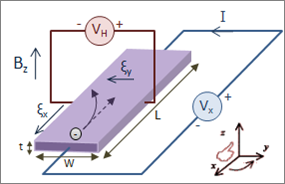
\includegraphics[scale=1.2]{hall.png}
\caption{Hall effect measurement setup for electrons. In steady-state the electrons follow the dashed straight arrow.  \cite{hall}}
\end{figure}


"The Hall coefficient is defined as the ratio of the induced electric field to the product of the current density and the applied magnetic field. It is a characteristic of the material from which the conductor is made, since its value depends on the type, number, and properties of the charge carriers that constitute the current." \cite{hall}

\begin{equation}
R_{H}= \dfrac{E_{y}}{J_{x}B_{z}}= \dfrac{V_{H}t}{I_{x}B_{z}}=\dfrac{1}{ne}
\end{equation}

which allows the measurement of both carriers density, applying a voltage across the x-axis, choosing positive or negative direction according to the carrier to be measured.



\section{Magnetoresistance}
The change in electrical resistivity of a metal when applying an external magnetic field is called magnetoresistance. Since in steady state all the forces are in
equilibrium, there is no transverse magnetoresistance. \cite{appendix}
Also assuming $B_{x}$ instead, the electrons are not affected by the Lorentz force and the longitudinal magnetoresistance cannot be explained. For this reason we have to consider the hole current too, thus we express the electric field for both carriers as $\vec{E} = \rho_{0,i} \vec{J}_{i} + \dfrac{e \tau _{i} \vec{B}}{m_{i}} \times \rho_{0,i} \vec{J}_{i}$ where $\rho_{0}$ is the zero field resistivity and the second term describes the induced Hall electric field.\

The current density of each carrier is given by $\vec{J}_{i}=\sigma _{i} \dfrac{E-\beta _{i}\vec{B} \times \vec{E} }{1+ \beta _{i}^{^{2}} B^{2}}$, with $\beta _{i}= \dfrac{e \tau _{i}}{m_{i}}$.\

The total current density now will be $\vec{J}_{tot}= \vec{J}_{1} + \vec{J}_{2}$, where $i=1,2$, thus we obtain 
 
\begin{equation}
\vec{J}_{tot}= \left( \dfrac{\sigma _{1}}{1+ \beta _{1}^{^{2}} B^{2}}    +  \dfrac{\sigma _{2}}{1+ \beta _{2}^{^{2}} B^{2}}   \right) \vec{E} -  \left( \dfrac{\sigma _{1} \beta _{1}}{1+ \beta _{1}^{^{2}} B^{2}}    +  \dfrac{\sigma _{2} \beta _{2}}{1+ \beta _{2}^{^{2}} B^{2}}   \right) \vec{B} \times \vec{E}
\end{equation}


The transverse magnetoresistance $\rho$ is given by connecting $\vec{J}$ with $\vec{E}$
in the direction of the total current as $\rho= \vec{J} \vec{E}/ J^{2}$. Comparing with  the specific resistivity without magnetic field $\rho _{0}= \dfrac{1}{\sigma _{1} + \sigma _{2}}$, we obtain 

\begin{equation}
\dfrac{\Delta \rho}{\rho}  = f \left[ \dfrac{B}{\rho_{0}}\right]
\end{equation}\label{Eq:magres}

where $\Delta \rho = \rho - \rho_{0}$ and always positive. Eq.\ref{Eq:magres} holds only for the calculation of the transverse magnetoresistance, since the derivation of the longitudinal requires a more complex model. The existence of magnetoresistance requires two types of carriers, where assuming that both have the same relaxation time $\tau$, the  magnetoresistance was derived as an approximate function of $\tau$ and B, known as the Kohler's Rule, depending on the type of metal only.



\section{Thermal conductivity }


In gases the transfer heat is conducted through direct collisions between molecules, thus their thermal conductivity is low compared to most solids (since they are dilute media). Non-metallic solids transfer heat by lattice vibrations so that there is no net motion of the media as the energy propagates through. Such heat transfer is often described in terms of "phonons", quanta of lattice vibrations. Metals are much better thermal conductors than non-metals because the same mobile electrons which participate in electrical conduction also take part in the transfer of heat.


For metals, the thermal conductivity is quite high, and those metals which are the best electrical conductors are also the best thermal conductors. At a given temperature, the thermal and electrical conductivities of metals are proportional, but raising the temperature increases the thermal conductivity while decreasing the electrical conductivity. This behaviour is quantified in the Wiedemann-Franz Law: $\kappa= L \sigma T$, where $L=\dfrac{\pi^{2}K^{2}_{_{B}}}{3e^{^{2}}}$ is the Lorentz number. Qualitatively, this relationship is based upon the fact that the heat and electrical transport both involve the free electrons in the metal. The thermal conductivity increases with the average particle velocity since that increases the forward transport of energy. However, the electrical conductivity decreases with particle velocity increase because the collisions divert the electrons from forward transport of charge. This means that the ratio of thermal to electrical conductivity depends upon the average velocity squared, which is proportional to the kinetic temperature as $T=\dfrac{mv^{2}}{3 K_{B}}$.\\

Here the electrical component of the thermal conductivity is described by $\kappa= \dfrac{\pi^{2} \tau n K_{B}^{2} T}{3m}$.\\


Wiedemann-Franz Law can be understood by treating the electrons like a classical gas and comparing the resultant thermal conductivity to the electrical conductivity, finally through $\dfrac{\kappa}{\sigma}= \dfrac{4 K_{B}^{2} T}{\pi e^{2}}$. \cite{wieman} \\
 $L = 2.23$ for copper at 0. Above Debye temperature L is again constant.



$T_{D}=347 K$  at 0K and $T_{D}=310$ at 290K.
\subsection{Debye Temperature}
The density of states for "phonons", is of the same form as the photon density of states in a cavity, Debye used a maximum allowed phonon frequency  $v_{D}$. In the treatment of specific heat, we define Debye temperature by $T_{D}=hv_{D}/K_{B}$.


\subsection{Fermi energy}
At higher than zero temperatures, the contribution of phonon to thermal transport in a system becomes important. The Fermi energy is the maximum energy occupied by an electron at 0K. By the Pauli exclusion principle, we know that the electrons will fill all available energy levels, and the top of that "Fermi sea" of electrons is called the Fermi energy or Fermi level. From the Fermi energy we can calculate the free electron density.


\begin{equation}
E_{F}= \dfrac{(hc)^{2}}{8mc^{2}} ( \dfrac{3n}{\pi})^{2/3}
\end{equation}


\subsection{Under magnetic field}
The conduction electrons in metals are the main carriers of the heat transportation similarly to the charge carriers.
Assuming a heat flow in the x-axis respectively to the case of the electron current and external $B_{z}$, the Lorentz force will again deflect the electrons in the y-axis direction, causing a reduction of the thermal conductivity in x direction. Thus the dependence of the thermal conductivity according to the magnetic field, similarly to the resistivity will be an approximate metal specific function $g$ of B and T.
\begin{equation}
\dfrac{\Delta \kappa }{\kappa }  = g \left[ \dfrac{B \kappa_{0}}{T}\right]
\end{equation}

Here $\kappa_{0}$ is the zero field thermal conductivity.












\section{Measuring Electric and thermal conductivity}

\subsection{Electrical resistivity (4-wire resistance measurement)\cite{4point}}

The electrical resistance is given by $R=V/I$, while the resistivity by $\rho= \lambda \dfrac{V}{I}$ where $\lambda$ is the geometric factor of the sample. To calculate the resistivity, we apply a constant current to the sample and then measure the voltage drop. If the electrical contacts of the Voltmeter have the same resistance with the sample, then we have to separate the contacts conducting the current from the contacts between the sample is measured, inorder not to measure the contact resistance along with the sample's.

\begin{figure}[H]
\centering
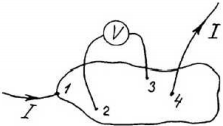
\includegraphics[scale=0.8]{4point.PNG}
\end{figure}

To avoid this we use the 4-point method that
allows to measure the voltage nearly currentless by a voltmeter connected directly to the sample. The resistivity is then determined by $\rho= \lambda \dfrac{V_{2-3}}{I_{1-4}}=\lambda \dfrac{V_{1-4}}{I_{2-3}}$.

In our case $\rho= A \dfrac{V_{2-3}}{I_{1-4} l}$, with $A$ the cross section area and $l$ the distance between the ............?????????

\subsection{Thermal conductivity (Steady-state method)}

The temperature gradient is measured by
a thermo couple. We similarly use a 4-point measurement method.\

j is the heat flux , heat power $P=V_{hp}I_{hp}$, A is the cross-sectional area, related as : $j_{x}= P/A $. $\Delta T$ is the temperature difference between the tips of the thermocouple, their distance $l$, we obtain the temperature gradient 
\begin{equation}
\Delta T_{_{tc}} /l_{tc} = \dfrac{V_{hp}I_{hp}}{A \kappa}
\end{equation}

Substituting $\Delta T_{tc}= V_{tc} / S$ we obtain 
\begin{equation}
\kappa = \dfrac{V_{hp} I_{hp} S l_{tc}}{V_{tc} A}
\end{equation}

\section{without magnetic field \cite{1}}
The noble metals (Cu, Ag, Au) are the most convenient materials for studying the transport properties of electrons in metals, because their Fermi surfaces have been investigated thoroughly and are sufficiently
simple for a rigorous theoretical analysis of the transport effects. The Fermi surfaces of each of these metals
are spheres linked by necks in the [111] directions.\\



At low temperatures ($T=0$) the electrical resistivity $\rho (T)$ is governed mainly by the scattering of electrons on static defects,
electrons, and lattice vibrations:

\begin{equation}
\rho (T)=  \rho_{0} + CT^{2} + AT^{5} 
\label{eq:1}
\end{equation} 

where $\rho_{0}$ is the residual resistivity due to the scattering of
electrons by static defects, $ CT^{2}$ and $AT^{5}$ are the resistivities
associated with the electron-electron and electron-phonon scattering processes, respectively.\

The electron-electron scattering is observed clearly only in the case of samples of extreme purity and is the
main process at sufficiently low temperatures. Magnetic impurities change the dependence $\rho (T)$ because of the Kondo effect. $A$ rises on increase
in $\rho _{0}$. At temperatures below 7 K (corresponding to $CT^{2} = AT^{5}$) the electron-electron
scattering in copper dominates the temperature dependence of the electrical resistivity.\\

The thermal resistivity W is governed at low temperatures mainly by the scattering of electrons on static defects, the scattering of electrons on phonons, and at sufficiently
low temperatures also by the scattering of electrons on other electrons
\begin{equation}
WT=\rho_{0}/L + DT^{2}+ BT^{3}
\end{equation}
where $L = 2.445 \cdot 10^{-8} W\Omega K^{-2}$ is the Lorenz constant, $DT$ is the thermal resistivity associated with the scattering of electrons
by other electrons, $BT^{2}$ is the resistivity due to the scattering of electrons by phonons.  $WT_{(T=0)}= \rho_{0}/L $. The contributions made by the electron-electron scattering
to the electrical resistivity and to the thermal resistivity are mutually related and the average value is $C/D = 0.92\cdot 10^{-8} W\Omega K^{-2}$ obtained by Lawrence. The contribution of the electron-phonon scattering (BT) depends on the value of $\rho_{0}$.

There was a correlation between the
contribution of the electron-electron scattering (coefficients C and D ) and the orientation of the investigated sample. The smallest values of C and D were obtained for the samples
oriented along the [111] axis. This result was unexpected because the transport coefficients of metals with the cubic lattice should not have been anisotropic.

\chapter{Analysis}

\chapter{Appendix}

\section{Error propagation formulas}

The error propagation for the calculated quantities $\lambda = f(\chi ,\psi)$ with the respective errors $ \delta\chi$ and $ \delta\psi$ was given by $\delta\lambda = \sqrt{(\dfrac{\partial \lambda}{\partial \chi} \delta\chi)^{2}+(\dfrac{\partial \lambda}{\partial \psi} \delta\psi)^{2}}$.\

For a mean value $ \eta =\dfrac{1}{N} \sum_{i=1}^{N} \eta _{i} $, the standard deviation is $\delta \eta = \sqrt{\dfrac{(\sum_{i=1}^{N} \eta _{i}- \eta  )^{2}}{N(N-1)}}$




\begin{equation*}
\Delta Res_{c} = \dfrac{\Delta lenght }{pixels} 
\end{equation*}

\begin{equation*}
\Delta_{length} =  \Delta Res_{c} \cdot pixels 
\end{equation*}
 
\begin{equation*}
\Delta A =  \Delta r \cdot 2 \pi r 
\end{equation*}










\begin{thebibliography}{99}


\bibitem{1} Transport properties of copper and silver
0. E. Omel'yanovskii, N. V. Zavaritskii, N. V. Lichkova, and V. N. Matveev
S. I. Vavilov Institute of Physics Problems, Academy of Sciences of the USSR, Moscow
(Submitted 15 March 1985)
Zh. Eksp. Teor. Fiz. 89,696-709 (August 1985)

\bibitem{drude} \url{http://www.physics.iisc.ernet.in/~aveek_bid/PH208/Lecture\% 201\%20Drude\%20model.pdf}


\bibitem{appendix} M 2.3 - Transport Properties of Copper, Appendix.

\bibitem{lore} \url{https://en.wikipedia.org/wiki/Lorentz_force}

\bibitem{hall} \url{https://en.wikipedia.org/wiki/Hall_effect}


\bibitem{4point} \url{https://www.iiserkol.ac.in/~ph324/StudyMaterials/GeometricFactors4ProbeResistivity.PDF}

\bibitem{wieman} \url{http://hyperphysics.phy-astr.gsu.edu/hbase/thermo/thercond.html}


\bibitem{references} \url{http://hyperphysics.phy-astr.gsu.edu/hbase/Tables/thrcn.html#c2}

\end{thebibliography}






\end{document}
